\documentclass[tikz,border=2mm]{standalone}
\usetikzlibrary{matrix,backgrounds,positioning,}

\begin{document}
	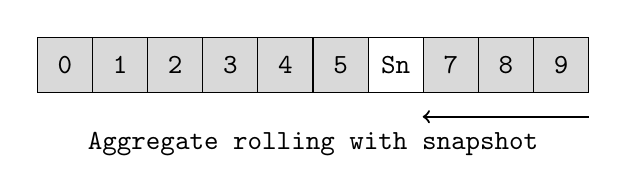
\begin{tikzpicture}[
	font=\ttfamily,
	array/.style={matrix of nodes,nodes={draw, minimum size=7mm, 
	fill=gray!30},column sep=-\pgflinewidth, row sep=0.5mm, nodes in empty cells
		}]
%	array/.style={matrix of nodes,nodes={draw, font=\ttfamily\scriptsize,minimum 
%	size=7mm, 
%	fill=gray!30},column sep=-\pgflinewidth, row sep=0.5mm, nodes in empty 
%cells}]
	
%	\matrix[array] (array) {
%		0 & 1 & 2 & 3 & 4 & 5 & 6 & 7 \\
%		0 & 1 & 2 & 3\\
%		0 & 1 & 2 & 3 & 4 & 5 & 6\\
%		0 & 1 & 2 & 3 & 4 \\};
%	
%		\matrix[array, below =of array] (array2) {
%			0 & 1 & 2 & 3 & 4 & 5 & 6 & 7\\
%			0 & 1 & 2 & 3\\
%			0 & 1 & 2 & 3 & 4 & 5 & 6\\
%			0 & 1 & 2 & 3 & 4 \\};
%	
%%		\matrix[array, below =of array2] (array3) {
%%			0 & 1 & 2 & 3 & 4 & 5 & 6 & 7 \\
%%			0 & 1 & 2 & 3\\
%%			0 & 1 & 2 & 3 & 4 & 5 & 6\\
%%			0 & 1 & 2 & 3 & 4 \\};
%	
%	\draw (-2.9,-1.7) rectangle (4,1.7) ;
%	\draw (-2.9,-6) rectangle (4,-2.5) ;
%%	\draw (-2.9,-10.3) rectangle (4,-6.7) ;
%	
%	\node[] at (2.7,-1.4) {\textit{Event Store A}};
%	\node[] at (2.7,-5.7) {\textit{Event Store B}};
%%	\node[] at (2.7,-10) {\textit{Event Store C}};

\matrix[array] (array) {
	0 & 1 & 2 & 3 & 4 & 5 & 6 & 7 & 8 & 9\\};


%%% WITH %%%
\node[draw, fill=white!20, minimum size=7mm] at (array-1-7) (box) {Sn};

\draw[<-,thick]([yshift=-3mm]array-1-8.south west) -- 
([yshift=-3mm]array-1-10.south east);
\node[align=center] at (0,-1) 
{Aggregate rolling with snapshot} ;


%%% WITHOUT %%%
%\draw[<-,thick]([yshift=-3mm]array-1-1.south west) -- 
%([yshift=-3mm]array-1-10.south east);
%\node[align=center] at (0,-1) 
%{Aggregate rolling without snapshot} ;

%%% WITHOUT %%%
%\draw[->,thick]([yshift=-3mm]array-1-1.south west) -- 
%([yshift=-3mm]array-1-10.south east);
%\node[align=center] at (0,-1) 
%{Aggregate} ;

	%
	\end{tikzpicture}
\end{document}